\newpage

\section{Control Theory}
\subsection{Introduction}
A controller is an essential part of most autonomous systems. This project is no exception - having control over where the pan and tilt system is pointing at is crucial to meeting the specified requirements.

When discussing what controller to use, figure \ref{fig:Standartsystem} is the point of reference, where the plant is the previously estimated transfer function, of the DC motor used in the system:

\begin{equation}
G(s)=\frac{105}{0.009s^2+s} \frac{[tachs/sec]}{[V]}
\end{equation}

\begin{figure}[h!]
\centering
\includegraphics[scale=0.5]{Billeder/Standartsystem.png}
\caption{ A generic way of representing a closed-loop control system }
\label{fig:Standartsystem}
\end{figure}

\newpage

\subsection{Controller selection}
For the sake of simplicity Proportional (P), Proportional-Integral (PI), Proportional-Derivative (PD) and Proportional-Integral-Derivative (PID) was the only controllers taken into consideration for this project. Lead-Lag compensators could be considered as well, since in essence they can have similar functionality.\par

A PID controller is made up by three parts: the proportional gain looks at the current error, the integral looks at the past errors and the derivative looks at current rate of change. Each term has a tuneable gain called the K constants. In general, these constants are what defines a PID controller’s behavior. See figure \ref{fig:PID controller} for illustration. 

\begin{figure}[h!]
\centering
\includegraphics[scale=0.5]{Billeder/PIDcontroller.png}
\caption{ A representation of the PID controller principle }
\label{fig:PID controller}
\end{figure}

This is the equation of the standard PID controller in the time domain:

\begin{equation}
K_{p}e(t)+K_{i} \int\limits_0^t \mathrm{e}(t)\,\mathrm{d}t+K_{d}\frac{de(t)}{dt}
\end{equation}

If transformed to the s domain the equations looks like this:\\

\begin{equation}G(s)=K_{p}+\frac{K_{i}}{s}+K_{d}s=\frac{K_{p}s+K_i+K_{d}s^2}{s}
\label{Eq_2}
\end{equation}

\subsubsection{Proportional Controller}

The P controller is by far the most straightforward controller, being that it is simply adding a gain to the open-loop transfer function. A P controller is a desired controller, since it is very simple to implement and tune, though this project have to meet the stated requirements.\par

To help analyse and give some intuition about how the motor’s transfer function behaves, a root locus of the open-loop transfer function is plotted see figure \ref{fig:RlocusControllers}. As one would expect it seems like this kind of controller will not suffice for the project.\par

As seen in figure \ref{fig:PStep}, the step response of the closed-loop transfer function, has an overshot of 14.1\%, and a settling time of 0.055 seconds. Meeting the specified requirements for the project with this controller is not possible. The overshoot can be decreased by reducing the gain below 1, but this induces a longer settling time and vice-versa. 

\begin{figure}[h!]
\centering
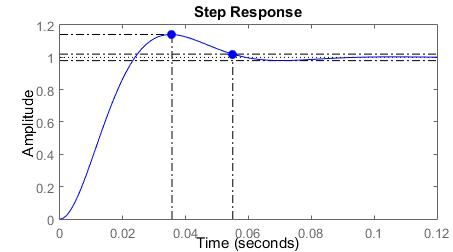
\includegraphics[scale=0.7]{Billeder/PStep.jpg}
\caption{ Peak amplitude: 1.14 - Overshot(\%): 14.1 - At time(seconds): 0.0356
		 Settling time (seconds): 0.055 }
\label{fig:PStep}
\end{figure}

\subsubsection{Proportional-Integral Controller}

The PI controller accumulates past error terms over time to eliminate steady-state errors in the system. This can cause an increase in overshoot called the integrator wind-up, and an increase in settling time. Though if a requirement is complying with a steady-state error of 0, then it is up to the designer to decide, if reaching steady-state is more vital to the system, than having more overshoot and a longer settling time.\par

Using a PI controller is the same as adding a pole and a zero to the open-loop transfer function. As seen in figure \ref{fig:RlocusControllers}, this controller does not seem to live up to the requirements either. Placing the zero and pole differently could make a better controller, but it would never be able to adjust to both design criteria.\par

The step response of the PI controller is seen on figure \ref{fig:PIStep}, the only difference from the P controller is a slightly longer peak time and settling time and a larger overshoot, as expected. This controller would not meet the requirements. 

\begin{figure}[h!]
\centering
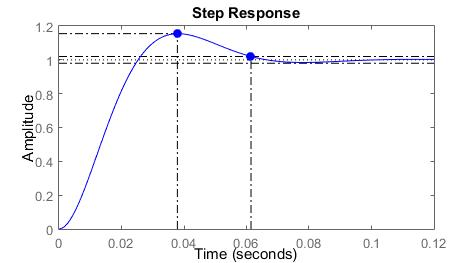
\includegraphics[scale=0.7]{Billeder/PIStep.jpg}
\caption{ Peak amplitude: 1.15 - Overshoot(\%): 15.5 - At time(seconds): 0.0379
		 Settling time (seconds): 0.0614 }
\label{fig:PIStep}
\end{figure}

\subsubsection{Proportional-Derivative Controller}

A PD controller is equivalent to the addition of a simple zero, which improves the transient response. From a different point of view, the PD controller may also be used to improve the settling time or stability, because it anticipates large errors and attempts corrective action before they occur. 

Figure \ref{fig:RlocusControllers} shows a promising root locus of the PD controller, it seems like that with the right amount of gain the system would fulfill the requirements.

The step response on figure \ref{fig:PDStep} shows, that in fact this controller would be ideal for this project. There is no overshoot, and the settling time is well below 0.05 seconds.

\begin{figure}[h!]
\centering
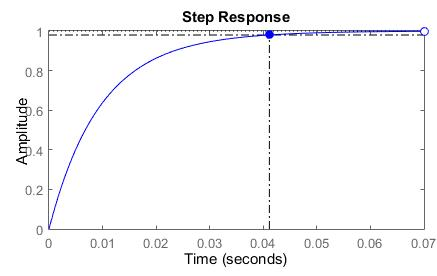
\includegraphics[scale=0.7]{Billeder/PDStep.jpg}
\caption{ Peak amplitude: $>$= 0.998 - Overshoot(\%): 0 - At time(seconds): $>$ 0.07
		 Settling time (seconds): 0.0411 }
\label{fig:PDStep}
\end{figure}

\subsubsection{Proportional-Integral-Derivative Controller}

The PID controller is the most complex controller which is going to be discussed. As noted earlier a PD controller was sufficient for generating the wanted response. So why discuss the PID? The reason is that real world systems might have limitations that the analysis have not taken into account yet. Reaching a steady-state error of 0 is actually a problem with a PD controller for this project, since the pan and tilt system does not function below a certain range of voltage, which means that an integral is needed.\par

Notice on figure \ref{fig:RlocusControllers}, that a PID controller is the addition of 2 zeros and 1 pole to the open-loop transfer function. The root locus shows that this system with a relative gain still meets the requirements of the design.\par

The step response of the PID controller, figure \ref{fig:PIDStep}, shows that indeed a PID controller would be a good choice of controller for this project. There is well below 10\% overshoot and the settling time is a great deal below 0.05 seconds.

\begin{figure}[h!]
\centering
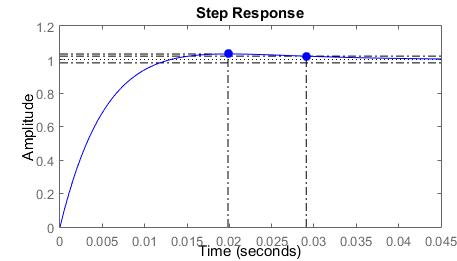
\includegraphics[scale=0.7]{Billeder/PIDStep.jpg}
\caption{ Peak amplitude: 1.03 - Overshot(\%): 2.92 - At time(seconds): 0.0201
		 Settling time (seconds): 0.0277 }
\label{fig:PIDStep}
\end{figure}

\begin{figure}[h!]
\centering
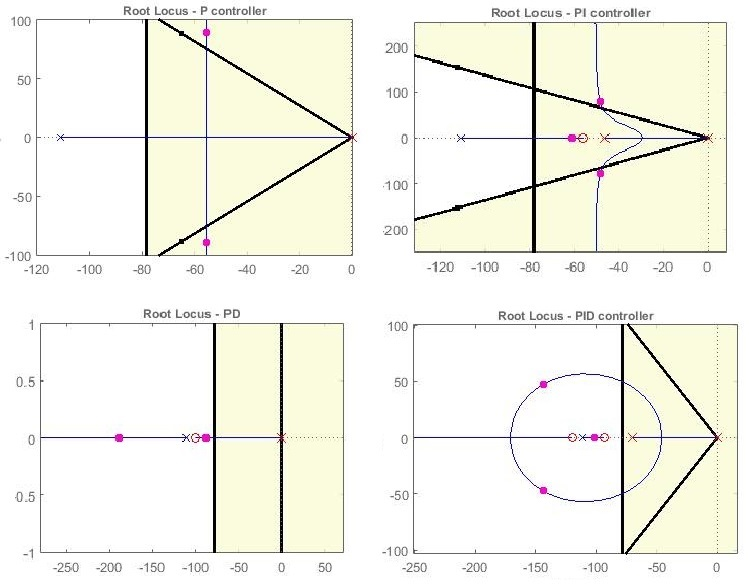
\includegraphics[scale=0.7]{Billeder/RlocusControllers.jpg}
\caption{ Open-loop transfer function Root Locus plots of the estimated motor transfer function, with different controllers. The shaded areas indicates unsatisfied design specifications, if poles of the closed-loop transfer function are placed there. 
The designs are: Overshoot $>$ 10\%, settling time $<$ 0.05 seconds. }
\label{fig:RlocusControllers}
\end{figure}


\subsection{K constants}

Once either a P, PI, PD or PID controller has been chosen for the project, the next step would be the estimation of K-constants for the respective controller. Finding these constants to meet one's requirements can be done in various ways. In this section the Manual tuning and Root Locus method will be discussed.


\subsubsection{Manual tuning}

This method requires the system to be online and running for tuning, though if a simulation of the system has been made this tuning method is still viable on the simulation - the catch is that a simulation’s artificiality cannot be denied, thus the actual online system proves more truthful.\par

There is no right way to tune manually, since experience can lead to a quick tuning. A known procedure is, however, to first set one’s $k_i$ and $k_d$ to zero, and then increase the $k_p$ until the system starts to oscillate, $k_p$ should then be set to approximately half this value. The $k_i$ is now increased to correct for any offset within the desired time. Lastly, if needed, the $k_d$ is increased until the requirements are met.


\subsubsection{Root Locus tuning method}

This method is a mathematical approach with the help of software like MatLab to find $k_p$, $k_i$ and $k_p$ from the root locus. It is not required to have the online system up and running to use this method, which in many cases can prove useful (imagine a system where unpredicted behavior can have fatal consequences). Though a mathematical model of the system is needed.\par

The root loci on figure \ref{fig:RlocusControllers} can be used, since they are the open-loop transfer function of the system. It has already been established that using a PID controller would be a good choice to meet the project’s requirements. Therefore this example is based on the PID root locus from figure \ref{fig:RlocusControllers}. The root locus was made with the SISO tool from Matlab with the open-loop transfer function equation \ref{eq:PosTF}. The two zeros at -90 and -55 on the real axis and a zero at the origin is what makes up the PID controller, and they were placed there to satisfy the design requirements. The SISO tool Compensator Editor of this root locus shows these zeros and pole as a compensator, which is another way to represent a PID controller. In the example of the PID controller from figure \ref{fig:RlocusControllers}  the compensator looks like this:\\ 

\begin{equation}
200\frac{(1+0.011s)(1+0.019s)}{s}
\label{Eq_1} 
\end{equation}

Rewriting equation \ref{Eq_1} to look like equation \ref{Eq_2} makes it quite easy to read the K constants.

\begin{equation}
\frac{0.0396s^2 +5.8s+200}{s}
\label{Eq_3}
\end{equation}

As seen in \ref{Eq_3} the K constants for the PID controller are $K_P$ = 5.8, $K_I$ = 200 and $K_D$ = 0.0396.

\subsubsection{Controller constants for Pan and Tilt systems}

Applying the root locus method to the transfer functions for the Pan and Tilt systems, PD and PID controller constants were derived for both of these. These constants can be found in figure \ref{fig:PIDControllerTable}.

\begin{figure}[h!]
\centering
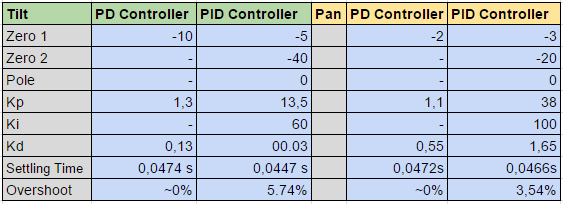
\includegraphics[scale=0.7]{Billeder/PIDControllerTable.png}
\caption{Table with K constants for PD \& PID controllers for the Pan- and Tilt systems}
\label{fig:PIDControllerTable}
\end{figure}

\subsection{Simulation}

Making a simulation of the system is a good way to figure out whether the controller needs to be redesigned or tweaks needs to taken into consideration. Since the motors on the pan and tilt are expected to have similar characteristic as the load free motor (though pan and tilt are expected to have different time constants), the simulation is then first done on the load free motor transfer function with the PD controller from figure \ref{fig:RlocusControllers}. The K constants were found with the same method as discussed in the Root Locus tuning Method section. The constants are $K_P = 2$ and $K_D = 0.02$.
The simulation is done in MatLab’s Simulink software, see figure \ref{fig:Simulinkmodel}. The Step block is a step input of 1, and since the DC gain of the plant is in the units of $\frac{tacs}{s V}$, this simulation illustrates the system rotating the motor 1 $tach$. The step input is fed to the feedback summation, where the feedback is subtracted from the reference input. The summation result is now the error signal, and this signal is then fed into the PD controller. The PD controller reacts depending on the rate of change of the error signal and passes on its calculated value. The motor plant produces physical rotation, which is integrated to $tachs$. The output is now sampled as feedback and is then fed back to the reference signal. The Time Scope will generate the plot of the simulation.

\begin{figure}[h!]
\centering
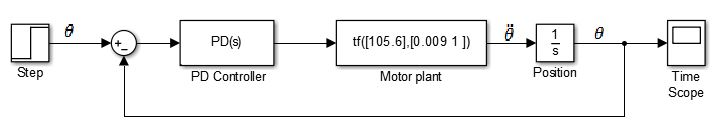
\includegraphics[scale=0.7]{Billeder/simulinkmodel.jpg}
\caption{ A simulink simulation of a PD controller of the load free motor’s transfer function. }
\label{fig:Simulinkmodel}
\end{figure}

The step response of the simulation is expected to look like the step response from the PD analysis. As seen on figure \ref{fig:SimuStepPDNoConstrains}, it looks a lot like expected. Upon inspecting the time 0.0226 seconds, the amplitude is 0.982 which is within 2\% of the settling time, so the simulation is very close to the expected.

\begin{figure}[h!]
\centering
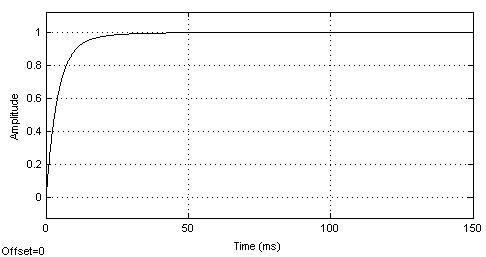
\includegraphics[scale=0.7]{Billeder/SimuStepPDNoConstrains.jpg}
\caption{ The step response of the simulation from figure \ref{fig:Simulinkmodel} }
\label{fig:SimuStepPDNoConstrains}
\end{figure}

Since this is a simulation of the physical system, the physical aspects that are obvious should be taken into consideration. The motor of the system cannot take inputs higher than 12 volts, therefore a saturation limit will be added to the PD controller to simulate this. Other than that, the friction and inertia in the system makes it impossible for the system to move below 2 volts. This means that inputs ranging from -2 volts to +2 volts to the plant, must always be set to 0 to simulate the idling of the motor. On figure \ref{fig:simulinkmodelwithconstrains} these changes can be seen.

\begin{figure}[h!]
\centering
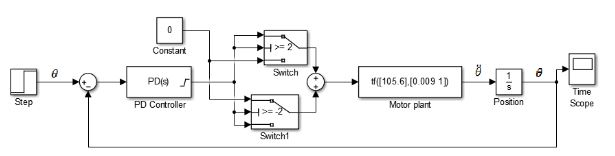
\includegraphics[scale=0.7]{Billeder/simulinkmodelwithconstrains.jpg}
\caption{ A Simulink simulation of a PD controller of the load free motor’s transfer function with saturation of -12 and +12 voltage and constraints with output 0 at voltage range -2 to +2 volts . }
\label{fig:simulinkmodelwithconstrains}
\end{figure}

The step response of figure \ref{fig:simulinkmodelwithconstrains} is seen on figure \ref{fig:SimuStepPDWithConstrains}, and as it is seen that the motor stops before reaching the target. This means in reality, the motor never reaches the target, and since this is a secondary requirement this is something that would be nice to compensate for. Luckily a PID controller has been discussed. and the constants for it is already known, and this controller is ready for simulation. Figure \ref{fig:SimuStepPIDWithConstrains} is the step response of the simulation of the PID controller, with the constants found in the Root Locus tuning method section, in the same setup as figure \ref{fig:simulinkmodelwithconstrains}. The step response shows that with a PID controller the simulation now reaches the desired target while still having a settling time below 50 ms. In conclusion a controller for the load free motor has been designed and simulated to work for the desired requirements.


\begin{figure}[h!]
\centering
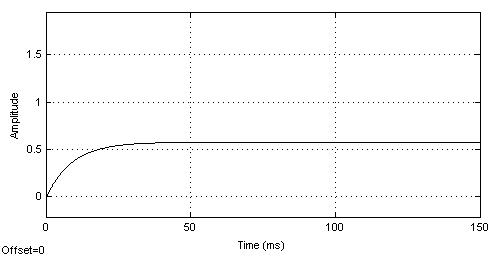
\includegraphics[scale=0.7]{Billeder/SimuStepPDWithConstrains.jpg}
\caption{ The step response of  the simulation from figure \ref{fig:simulinkmodelwithconstrains} with a PD controller }
\label{fig:SimuStepPDWithConstrains}
\end{figure}


\begin{figure}[h!]
\centering
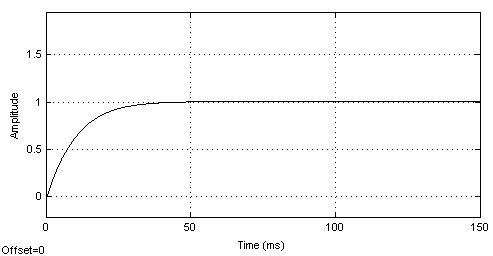
\includegraphics[scale=0.7]{Billeder/SimuStepPIDWithConstrains.jpg}
\caption{ The step of the simulation from \ref{fig:simulinkmodelwithconstrains} with a PID controller }
\label{fig:SimuStepPIDWithConstrains}
\end{figure}

Since the simulation of the load free motor needed a PID controller to meet the requirements, the pan and tilt motor on the actual system is expected to be of the same behavior, and would also need a PID controller. Also the system constrains on the system might prove of a problem for the PID controllers of the pan and tilt, since the saturation and the deadband between -2 volts and +2 volts, has not been take into considerations while designing the control system. The transfer functions of the pan and tilt were simulated in the same manner as in figure \ref{fig:simulinkmodelwithconstrains} with both PD and PID controller constants shown in figure \ref{fig:PIDControllerTable}.

On figure \ref{fig:SimuStepTiltPDAndPID} the step responses of the pan motor with PID and PD control can be seen, it is clear that, as expected, the PD control does not reach an acceptable steady state, while also being a lot slower than the required settling time of 50 milliseconds. The PID control however reaches an acceptable steady state. Nonetheless the settling time of 0.689 seconds is also too slow, and there is an overshoot of 11.2\%.

The slow settling time and overshoot can be explained by the saturation of the plant, and the deadband between -2 volts and +2 volts. The designed controllers do not compensate for these factors. 

\begin{figure}[h!]
\centering
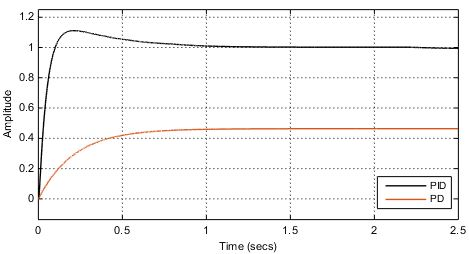
\includegraphics[scale=0.7]{Billeder/SimuStepPanPDAndPID.jpg}
\caption{ Step response of the simulation from figure \ref{fig:simulinkmodelwithconstrains} with pan motor and results of both PD and PID controllers.
 }
\label{fig:SimuStepTiltPDAndPID}
\end{figure}

Likewise on figure \ref{fig:SimuStepTiltPDAndPID}, the step responses of the tilt motor with PID and PD control can be seen. As expected the PD control never reaches an acceptable steady state, and the settling time is slower. The PID controller reaches an acceptable steady state, but also have a long settling time of 0.491, while also having an overshot of 18.7\%.
Same as for tilt motor, these behaviors can be explained by the saturation of the plant and the deadband between -2 volts and +2 volts.


\begin{figure}[h!]
\centering
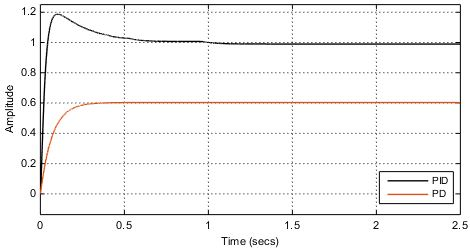
\includegraphics[scale=0.7]{Billeder/SimuStepTiltPDAndPID.jpg}
\caption{  Step response of the simulation from figure \ref{fig:simulinkmodelwithconstrains} with tilt motor and results of both PD and PID controllers.
 }
\label{fig:SimuStepTiltPDAndPID}
\end{figure}


Another simulation on the pan and tilt motors were run. This time an step input of 540 was set. This is equal to half a revolution on either motors. This simulation was run, because in practice,  the system should be able to handle the kind of inputs.
On figure \ref{fig:SimuStepPanAndTiltNoWindUpProtection} the step response of 540 can be seen, as noted the pan and motors overshoot with about 100\% and the settling time is greatly increased because of this. This happens because of integrator windup, and was not compensated for when designing the controllers. In the simulation an anti windup can be set, to simulate an implementation of windup protection. On figure \ref{fig:SimuStepPanAndTiltWithWindUpProtection} the result of a step input of 540 with windup protection on can be seen. The pan and tilt on figure \ref{fig:SimuStepPanAndTiltWithWindUpProtection} seems to behave acceptable, the tilt has no overshoot and the pan has an overshot of 3.4 \% overshoot. Though the settling time is still slow, however this is to be expected as the system is saturated.


\begin{figure}[h!]
\centering
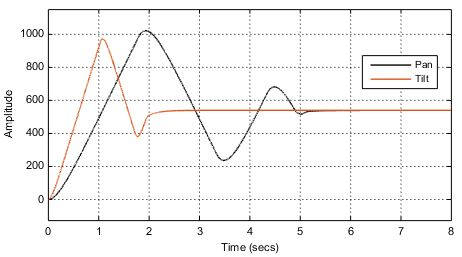
\includegraphics[scale=0.7]{Billeder/SimuStepPanAndTiltNoWindUpProtection.jpg}
\caption{  Step response of the simulation from figure  \ref{fig:simulinkmodelwithconstrains} and 540 input instead of 1. The pan and tilt motor are without wind up protection. }
\label{fig:SimuStepPanAndTiltNoWindUpProtection}
\end{figure}


\begin{figure}[h!]
\centering
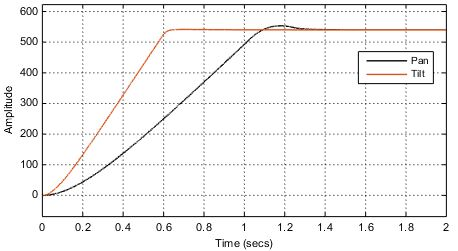
\includegraphics[scale=0.7]{Billeder/SimuStepPanAndTiltWithWindUpProtection.jpg}
\caption{   Step response of the simulation from figure \ref{fig:simulinkmodelwithconstrains} and 540 input instead of 1. The pan and tilt motor are with wind up protection on.
 }
\label{fig:SimuStepPanAndTiltWithWindUpProtection}
\end{figure}

The transfer functions and the controllers for the pan and tilt have now been tested in simulation, and the designed controllers seems promising. The tilt motor would on a small step input not fulfill the requirements of less than 10\% overshoot and the settling time requirement is not met either. It would seem like that reaching a settling time of 0.05 seconds or less would be impossible for the tilt, since the system cannot move fast enough. Tough for a step input of a larger scale, the overshoot is nigh zero and well within the requirement.
As for the pan motor, a small step input has an overshoot really close to 10\%, but a long settling time. The requirement of having overshoot less than 10\% is therefore not fulfilled, either is the having a settling time of 0.05 seconds for the pan motor. On a larger input the pan motor has an overshoot of only 3.4\% and is well within the requirement.

In general, the overshoot requirement of 10\% seems to met for step inputs of a relative size, and the settling time requirement of 50 ms is impossible for the system to meet, because of saturation and deadband.

\subsection{Implementation - digital}

\subsubsection{Direct implementation}

One way of implementing the controller is a direct implementation of the PID-controller. In this case, the plant input will be a summation of the 3 PID contributions, that will all have to be calculated in real-time. This method makes a lot of sense intuitively, and provides easy access to modifying the K-constants during the tuning-process, as these are simply constants that are multiplied with the 3 contributions. In order to use this method, the mathematical operations of integration and differentiation will be have to implemented.


\subsubsection{Filter approach}

An alternative way to implement the PID controller is converting it into a discrete-time filter. This method has the advantage of not having to do any actual integration or differentiation on the FPGA. Given a continuous-time transfer function and a sampling rate, the matlab command “c2d” can convert the transfer function to the z-domain. Through algebraically isolating the current output of the controller, the filter coefficients for the implementation can be calculated.\par

The sampling rate should ideally be as high as possible, as this will improve the accuracy of the discrete filter. Through matlab tests, it was found that sampling rates of higher than 10kHz do not create further improvement in the accuracy of the filter, and thus there was no need to increase the sampling rate beyond this value, even though it was technically possible.

\subsubsection{Discrete filter for Pan-system [10kHz]}

Using the above method, discrete filters were calculated for the Pan- and tilt systems.

\begin{equation}
\frac{u(z)}{e(z)}=\frac{1.65z^2-3.3z+1.65}{z^2-2z+1}=\frac{1.65-3.3z^-1+1.65z^-2}{1-2z^-1+z^-2}
\end{equation}

\begin{equation}
u(z)(1-2z^-1+z^-2)=e(z)(1.65-3.3z^-1+1.65z^-2)
\end{equation}

\begin{equation}
u[n]-2u[n-1]+u[n-2]=e[n]-3.3e[n-1]+1.65e[n-2]
\end{equation}

\begin{equation}
u[n]=e[n]-3.3e[n-1]+1.65e[n-2]+2u[n-1]-u[n-2]
\end{equation}

\subsubsection{Discrete filter for Tilt-system [10kHz]}

\begin{equation}
\frac{u(z)}{e(z)}=\frac{0.3z^2-0.5999z+0.2999}{z^2-2z+1}=\frac{0.3-0.05999z^-1+0.299z^-2}{1-2z^-1+z^-2} =>
\end{equation}

\begin{equation}
u(z)(1-2z^-1+z^-2)=e(z)(0.3-0.05999z^-1+0.299z^-2)
\end{equation}

\begin{equation}
u[n]-2u[n-1]+u[n-2]=0.3e[n]-0.05999e[n-1]+0.299e[n-2]
\end{equation}

\begin{equation}
u[n]=0.3e[n]-0.05999e[n-1]+0.299e[n-2]+2u[n-1]-u[n-2]
\end{equation}

\subsection{Overview}
The necessary coefficients and constants have been found to complete the implementation-method of choice. The discrete filter method, however, was discovered quite late in the chronology of the project, and due to this lacks verification and testing. Most of the project work has been carried out under the assumption that the direct implementation method was the best, and thus this method has been given the main focus during testing and implementation.